\chapter{Methodology}
\section{Introduction}
This chapter explain the procedure to achieve the objectives declared in the previous chapter. Each objective consist of a series of activities that produce an outcome, each one contributing to reach the general objective of this monograph. First, a description of the data pre-processing, then the selection of computer parameters and finally, a description of the methodology for training and testing the models. 
\section{Data analysis and pre-processing}
The dataset consists of two files, one with the redshift measurement of DESI (TAR file) and the other with simulated true redshifts (TRUTH file). Apart from this, the files also contain several variables related to the simulations parameters, the type of target, the observation conditions, etc. 
\begin{figure}[h!]
	\centering
	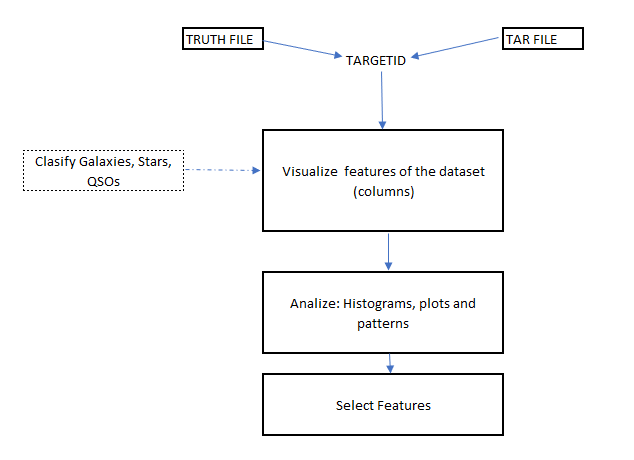
\includegraphics[width=1\linewidth]{TeX_files/Imagenes/metho_1}
	\caption{General methodology to understand the dataset and extract valuable features.}
	\label{fig:metho1}
\end{figure}
Figure \ref{fig:metho1} shows the general step-by-step method to understand the data. In the first step, the two files have to be linked by the variable TARGETID, this variable represent the identity of a target through the whole pipeline of the experiments (observation and measurements). After this, the next step is to discriminate by target type and observe the behavior of the other variables in the files. From this one can neglect some basic variables that give no relevant information to the problem. A second analysis can be executed with more details, to see if the variables hold any relation with the redshift measurement, using histograms and approximating distribution. This is done to select which variables (or features) can be used to explain the difference between the true redshift of a galaxy and the redshift measured by DESI. The details of this can be found in Chapter \ref{Ch:Data}. After the features are selected, they will be scaled so that the means are equal to zero and the variance to one. 

\section{High performance computing analysis}

The training time if the model depends on the size of the training set, however, since it is going to be executed in parallel in the computing cluster of the University, the training time will also depend on the resources of the hardware. For example, the memory of the machine and the number of processor in which the code will be parallelized, as well as the number of processor that the computer (or node) actually has. To see what is the best combination of parameters to train the models in a reasonable amount of time up to a reasonable accuracy, it will be necessary to restrict also the size of the dataset used for training.

\begin{figure}[h!]
	\centering
	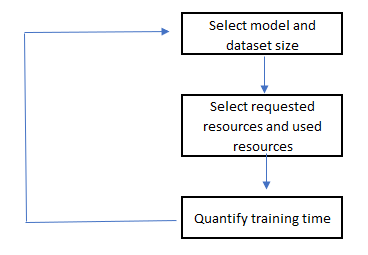
\includegraphics[width=0.7\linewidth]{TeX_files/Imagenes/metho_2}
	\caption{Sequence of step to gather enough information to understend the relation between computation time, memory, dataset size and processors.}
	\label{fig:metho2}
\end{figure}

Figure \ref{fig:metho2} shows the step to accomplish this. First, select the model and architecture (grid search / cross validation, explained next) and the dataset size, in order to see how the training time scales with size, it is necessary to select different sizes, in this case, 100, 1000, 5000, and 10000. Then, the algorithm have to be run in certain number of processors, and with certain RAM memory,in this case, we will try 1, 4, 8 and 16 processors, and 16, 32, 64 and 128 GB of memory. The expected result is number of parameters to run the complete training algorithm on a big dataset. 
\section{Machine Learning}
Once we understand the scalability of the training time with respect to hardware variables, it is time to train and test the models. For this the dataset will be divided in a training set, corresponding to 75\% of the dataset and a test set (the rest 25 \%) as shown in Figure \ref{fig:metho3}. After this, according to the results of the previous section, the training set will be split in subsets of specific size, this subsets will be again divided into a development and evaluation sets, to apply to them the grid search and cross validation. This two methods are used to select the hyper-parameters of the models and to quantify the error of the algorithms. 
\begin{figure}[h!]
	\centering
	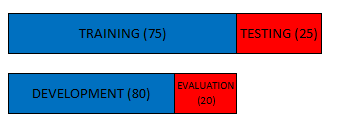
\includegraphics[width=0.6\linewidth]{TeX_files/Imagenes/metho_3}
	\caption{Divition of the dataset in train and test. The train set is divided in development-evaluation subsets.}
	\label{fig:metho3}
\end{figure}
\subsection{Training}
For training, we will use grid search and cross validation to select the hyper-parameters of the models.
The grid search method correspond to train the model with different combinations of parameters as in going over a grid, and search for the combinations of parameters that give the best results. This is used alongside cross validation, which consist on training the model several times by randomly assigning the development and the evaluation sets. Therefore, it reports the mean and standard error of the metrics of the trained models.
\subsection{Testing}
Once the models are trained, they will be test on the unseen 25\% of the data to check its generalization ability. This means, that we need to see whether the model truly 'learns' to predict redshifts or just memorized the training dataset. To select the best performing algorithm on the test dataset, the criterion will be the $r^2$ measure and the simplicity of the model.



In general, the methodology for this project consist in analysing the complete dataset and selecting the valuable features than can be used to predict a correct redshift, finding the scalability of the training time with respect to the size of the dataset and the cluster resources, an finally, training an evaluating the machine learning models. 




